\documentclass[a4paper,12pt]{article}

\usepackage{graphicx}
\usepackage{amsmath}
\usepackage{hyperref}
\usepackage{caption}
\usepackage{subcaption}
\usepackage{circuitikz}
\usepackage{tikz}

\begin{document}
\subsection{Design Examples}
\subsubsection{Three-Way Light Control}
\begin{itemize}
  \item Say there is a large room with 3 lights, with corresponding switches. Let $x_1, x_2, x_3$ denote the state of each switch.
  \item The light is $OFF$ when all switches are open. The light is $ON$ if exactly one switch is closed, and $OFF$ if two (or no) switches are closed.
  \item Let state of the light be represented by the function $f(x_1, x_2, x_3)$.
\end{itemize}
We shall try to represent$f(x_1, x_2, x_3)$ in sum-of-products form \newline
\textbf{Sum-of-Products Form}\newline
The function \( f \) is expressed as:
\begin{align*}
  f = m_1 + m_2 + m_4 + m_7 = \overline{x_1}x_2\overline{x_3} + x_1\overline{x_2}\overline{x_3} + \overline{x_1}\overline{x_2}x_3 + x_1x_2x_3
\end{align*}
This expression cannot be simplified further.
\begin{figure}[h!]
  \centering
  \resizebox{1\textwidth}{!}{%
    \begin{circuitikz}
      \tikzstyle{every node}=[font=\small]

      \draw (13.75,17) to[short] (14,17);
      \draw (13.75,16.5) to[short] (14,16.5);
      \draw (14,17) node[ieeestd and port, anchor=in 1, scale=0.89](port){} (port.out) to[short] (15.75,16.75);
      \draw (13.75,14.5) to[short] (14,14.5);
      \draw (13.75,14) to[short] (14,14);
      \draw (14,14.5) node[ieeestd and port, anchor=in 1, scale=0.89](port){} (port.out) to[short] (15.75,14.25);
      \draw (13.75,12) to[short] (14,12);
      \draw (13.75,11.5) to[short] (14,11.5);
      \draw (14,12) node[ieeestd and port, anchor=in 1, scale=0.89](port){} (port.out) to[short] (15.75,11.75);
      \draw (13.75,9.5) to[short] (14,9.5);
      \draw (13.75,9) to[short] (14,9);
      \draw (14,9.5) node[ieeestd and port, anchor=in 1, scale=0.89](port){} (port.out) to[short] (15.75,9.25);
      \draw (13.75,9) to[short] (3.75,9);

      \draw (14.35,9.25) to[short] (3.75,9.25);
      \draw (13.75,9.5) to[short] (3.75,9.5);
      \draw (7.5,9.5) node[ieeestd not port, anchor=in, rotate=-270](port){} (port.out) to[short] (7.5,11.5);
      \draw (port.in) to[short] (7.5,9);
      \draw (14.35 ,11.75) to[short] (7.5,11.75);
      \draw (7.5,11.25) to[short] (7.5,11.75);
      \draw (6.25,9.75) node[ieeestd not port, anchor=in, rotate=-270](port){} (port.out) to[short] (6.25,12);
      \draw (port.in) to[short] (6.25,9.25);
      \draw (6.25,12) to[short] (14,12);
      %\draw (5,9.75) node[ieeestd not port, anchor=in, rotate=-270](port){} (port.out) to[short] (5,12);
      %\draw (port.in) to[short] (5,9.25);
      \draw (5,12) to[short] (5,17);
      \draw (5,17) to[short] (14,17);
      \draw (14.35,16.75) to[short] (6.25,16.75);
      \draw (6.25,16.75) to[short] (6.25,11.75);
      \draw (13.75,14.5) to[short, -o] (5,14.5) ;
      \draw (14,12) to[short, -o] (6.25,12) ;
      \draw (14,11.75) to[short, -o] (7.5,11.75) ;
      \draw (7.5,11.75) to[short] (7.5,14);
      \draw (14.35,14.25) to[short] (7.5,14.25);
      \draw (7.5,14.25) to[short] (7.5,13.75);
      \draw (13.75,16.5) to[short] (8.75,16.5);
      \draw (8.75,16.5) to[short, -o] (8.75,9) ;
      \draw (13.75,14) to[short] (10,14);
      \draw (10,14) to[short, -o] (10,9.25) ;
      \node [font=\small, color={rgb,255:red,255; green,255; blue,255}] at (3.5,9.5) {$x_1$};
      \node [font=\small, color={rgb,255:red,255; green,255; blue,255}] at (3.5,9.5) {Text};
      \node [font=\small, color={rgb,255:red,255; green,255; blue,255}] at (3.5,9.5) {$x_1$};
      \node [font=\small, color={rgb,255:red,255; green,255; blue,255}] at (3.5,9.5) {Text};
      \node [font=\small, color={rgb,255:red,255; green,255; blue,255}] at (3.5,9.5) {Text};
      \node [font=\small, color={rgb,255:red,255; green,255; blue,255}] at (3.5,9.5) {Text};
      \node [font=\small, color={rgb,255:red,255; green,255; blue,255}] at (3.5,9.5) {Text};
      \node [font=\small, color={rgb,255:red,255; green,255; blue,255}] at (3.5,9.5) {Text};
      \node [font=\small, color={rgb,255:red,255; green,255; blue,255}] at (3.5,8.25) {Text};
      \node [font=\small] at (3.5,9.5) {$x_1$};
      \node [font=\small] at (3.5,9.25) {$x_2$};
      \draw (5,9.75) node[ieeestd not port, anchor=in, rotate=-270](port){} (port.out) to[short] (5,12);
      \draw (port.in) to[short] (5,9.5);
      \node [font=\small] at (3.5,9) {$x_3$};
      \draw (6.25,10) to[short, -o] (6.25,9.25) ;
      \draw (7.5,9.75) to[short, -o] (7.5,9) ;
      \draw (5,10) to[short, -o] (5,9.5) ;
      %\draw (15,9.25) to[short, -o] (17,9.25) ;
      \draw (13.75,11.5) to[short] (11.25,11.5);
      \draw (11.25,11.5) to[short, -o] (11.25,9.5) ;
      \draw (17,13.5) to[short] (17.25,13.5);
      \draw (17,13) to[short] (17.25,13);
      \draw (17.25,13.5) node[ieeestd or port, anchor=in 1, scale=0.89](port){} (port.out) to[short] (19,13.25);
      \draw (17,13.5) to[short] (17,16.75);
      \draw (15.75,16.75) to[short] (17,16.75);
      \draw (17,13) to[short] (17,9.25);
      \draw (17,9.25) to[short] (15.5,9.25);
      \draw (15.75,11.75) to[short] (16.25,11.75);
      \draw (15.75,14.25) to[short] (16.25,14.25);
      \draw (16.25,14.25) to[short] (16.25,13.25);
      \draw (16.25,11.75) to[short] (16.25,13.25);
      \draw (16.25,13.25) to[short] (17.6,13.25);
    \node [font=\small] at (19.3,13.25) {$f$};\end{circuitikz}
    }%

    \label{fig:sum-of-products}
    \caption{Sum-of-Products}
  \end{figure}\\
  \textbf{Product-of-Sums Form}\newline
  The function $f$ can also be expressed as:
  \begin{align*}
    f = M_0 \cdot M_3 \cdot M_5 \cdot M_6 = (x_1 + x_2 + x_3)(x_1 + \overline{x_2} + \overline{x_3})(\overline{x_1} + x_2 + \overline{x_3})(\overline{x_1} + \overline{x_2} + x_3)
  \end{align*}
  This form has the same cost as the sum-of-products realization.\newline
\begin{figure}[h!]
\centering
\resizebox{1\textwidth}{!}{%
\begin{circuitikz}
\tikzstyle{every node}=[font=\small]
\draw (10,15.75) to[short] (10.25,15.75);
\draw (10,15.25) to[short] (10.25,15.25);
\draw (10.25,15.75) node[ieeestd or port, anchor=in 1, scale=0.89](port){} (port.out) to[short] (12,15.5);
\draw (port.left) to[short] (10,15.5);
\draw (10,13.25) to[short] (10.25,13.25);
\draw (10,12.75) to[short] (10.25,12.75);
\draw (10.25,13.25) node[ieeestd or port, anchor=in 1, scale=0.89](port){} (port.out) to[short] (12,13);
\draw (port.left) to[short] (10,13);
\draw (10,10.75) to[short] (10.25,10.75);
\draw (10,10.25) to[short] (10.25,10.25);
\draw (10.25,10.75) node[ieeestd or port, anchor=in 1, scale=0.89](port){} (port.out) to[short] (12,10.5);
\draw (port.left) to[short] (10,10.5);
\draw (10,8.25) to[short] (10.25,8.25);
\draw (10,7.75) to[short] (10.25,7.75);
\draw (10.25,8.25) node[ieeestd or port, anchor=in 1, scale=0.89](port){} (port.out) to[short] (12,8);
\draw (port.left) to[short] (10,8);
\draw (10,15.75) to[short] (2.5,15.75);
\draw (10,15.25) to[short] (3.75,15.25);
\draw (3.75,15.25) to[short] (3.75,14.5);
\draw (3.75,14.5) to[short] (2.5,14.5);
\draw (10,15.5) to[short] (3.25,15.5);
\draw (3.25,15.5) to[short] (3.25,15);
\draw (10,8) to[short] (5,8);
\draw (10,7.75) to[short] (3.75,7.75);
\draw (3.75,7.75) to[short, -o] (3.75,14.5) ;
\draw (10,13) to[short, -o] (6.25,13) ;
\draw (10,8.25) to[short] (6.25,8.25);
\draw (10,10.75) to[short, -o] (5,10.75) ;
\draw (5,15.25) node[ieeestd not port, anchor=in, rotate=-90](port){} (port.out) to[short] (5,13.25);
\draw (port.in) to[short] (5,15.75);
\draw (6.25,15.25) node[ieeestd not port, anchor=in, rotate=-90](port){} (port.out) to[short] (6.25,13.5);
\draw (port.in) to[short] (6.25,15.5);
\draw (7.5,15) node[ieeestd not port, anchor=in, rotate=-90](port){} (port.out) to[short] (7.5,13.25);
\draw (port.in) to[short] (7.5,15.25);
\draw (10,12.75) to[short, -o] (7.5,12.75) ;
\draw (10,13.25) to[short, -o] (10,15.75) ;
\draw (8.75,10.5) to[short, -o] (8.75,15.5) ;
\draw (10,10.5) to[short] (8.75,10.5);
\draw (10,10.25) to[short] (7.5,10.25);
\draw (7.5,10.25) to[short] (7.5,13.25);
\draw (6.25,8.25) to[short] (6.25,13.75);
\draw (5,8) to[short] (5,13.25);
\draw (3.25,15) to[short] (2.5,15);
\draw (5,15) to[short, -o] (5,15.75) ;
\draw (13.75,12.25) to[short] (14,12.25);
\draw (13.75,11.75) to[short] (14,11.75);
\draw (14,12.25) node[ieeestd and port, anchor=in 1, scale=0.89](port){} (port.out) to[short] (15.75,12);
\draw (port.left) to[short] (13.75,12);
\draw (13.75,12.25) to[short] (13.75,15.5);
\draw (13.75,15.5) to[short] (12,15.5);
\draw (13.75,11.75) to[short] (13.75,8);
\draw (12,8) to[short] (13.75,8);
\draw (12,13) to[short] (13.25,13);
\draw (12,10.5) to[short] (13.25,10.5);
\draw (13.25,10.5) to[short] (13.25,12);
\draw (13.25,13) to[short] (13.25,12);
\draw (13.25,12) to[short] (13.75,12);
\node [font=\small] at (2,14.5) {$x_1$};
\node [font=\small] at (2,15) {$x_2$};
\node [font=\small] at (2,15.75) {$x_3$};
\node [font=\small] at (16,12) {$f$};
\end{circuitikz}
}%

\label{fig: Product-of-Sums}
\caption{Product-of-Sums}
\end{figure}\\
\textbf{Truth Table}\newline
  Truth table for the 3-way light control is as follows,
  \[
    \begin{array}{|c|c|c|c|}
      \hline
      x_1 & x_2 & x_3 & f(x_1, x_2, x_3) \\
      \hline
      0 & 0 & 0 & 0 \\
      0 & 0 & 1 & 1 \\
      0 & 1 & 0 & 1 \\
      0 & 1 & 1 & 0 \\
      1 & 0 & 0 & 1 \\
      1 & 0 & 1 & 0 \\
      1 & 1 & 0 & 0 \\
      1 & 1 & 1 & 1 \\
      \hline
    \end{array}
  \]
  \subsubsection{Multiplexer Circuit}
  \begin{itemize}
    \item In computer systems, it is often necessary to select data from exactly one of several sources.Consider two data sources, represented by input signals $x_1$ and $x_2$, which change over time.\\
    \item A circuit is needed to produce an output that matches either $x_1$ or $x_2$, depending on a selection control signal $s$. 
  \end{itemize}
  The circuit has three inputs: $x_1$, $x_2$, and $s$. The output $f$ is defined as:
  \begin{align*}
    f = \begin{cases}
      x_1 & \text{if } s = 0, \\
      x_2 & \text{if } s = 1.
    \end{cases}
  \end{align*}
  The Sum-of-Products form of the function is,
  \begin{align*}
    f(s, x_1, x_2) = s x_1 x_2 + s x_1 \overline{x_2} + \overline{s} x_1 x_2 + \overline{s} \overline{x_1} x_2.
  \end{align*}
  Using the distributive property,
  \begin{align*}
    f = \overline{s}x_1(\overline{x_2} + x_2) + s(\overline{x_1} + x_1)x_2
  \end{align*}
  Applying theorems of boolean algebra $x + \overline(x) = 1$,
  \begin{align*}
    f = s x_1 + \overline{s} x_2.
  \end{align*}
  \begin{itemize}
    \item A circuit implementing this function is called a \textbf{2-to-1 multiplexer}. It selects one of two data inputs $(x_1$ or  $x_2)$ based on the control signal $s$.\\
    \item Multiplexers are widely used in digital systems, and larger multiplexers (e.g., 4-to-1, 8-to-1) can be built by extending this concept. A 4-to-1 multiplixer would require two control signals, while an 8-to-1 multiplexer would require three.
  \end{itemize}
  The truth table for the 2-to-1 multiplexer is as follows:

  \[
    \begin{array}{|c|c|c|c|}
      \hline
      s & x_1 & x_2 & f(s, x_1, x_2) \\
      \hline
      0 & 0 & 0 & 0 \\
      0 & 0 & 1 & 0 \\
      0 & 1 & 0 & 1 \\
      0 & 1 & 1 & 1 \\
      1 & 0 & 0 & 0 \\
      1 & 0 & 1 & 1 \\
      1 & 1 & 0 & 0 \\
      1 & 1 & 1 & 1 \\
      \hline
    \end{array}
  \]
  A 2-to-1 multiplexer can be built using the basic $AND, OR, NOT$ gates
  \begin{figure}[!ht]
    \centering
    \resizebox{1\textwidth}{!}{%
      \begin{circuitikz}
        \tikzstyle{every node}=[font=\small]
        \draw (8.75,15.75) to[short] (9,15.75);
        \draw (8.75,15.25) to[short] (9,15.25);
        \draw (9,15.75) node[ieeestd and port, anchor=in 1, scale=0.89](port){} (port.out) to[short] (10.75,15.5);
        \draw (8.75,13.25) to[short] (9,13.25);
        \draw (8.75,12.75) to[short] (9,12.75);
        \draw (9,13.25) node[ieeestd and port, anchor=in 1, scale=0.89](port){} (port.out) to[short] (10.75,13);
        \draw (8.75,15.75) to[short] (5,15.75);
        \draw (8.75,15.25) to[short] (6.25,15.25);
        \draw (8.75,13.25) to[short] (5,13.25);
        \draw (8.75,12.75) to[short] (5,12.75);
        \draw (6.25,13.5) node[ieeestd not port, anchor=in, rotate=-270](port){} (port.out) to[short] (6.25,15.25);
        \draw (port.in) to[short] (6.25,13.25);
        \draw (11.75,14.75) to[short] (12,14.75);
        \draw (11.75,14.25) to[short] (12,14.25);
        \draw (12,14.75) node[ieeestd or port, anchor=in 1, scale=0.89](port){} (port.out) to[short] (13.75,14.5);
        \draw (10.75,15.5) to[short] (11.75,15.5);
        \draw (11.75,14.75) to[short] (11.75,15.5);
        \draw (11.75,14.25) to[short] (11.75,13);
        \draw (11.75,13) to[short] (10.75,13);
        \node [font=\small] at (14.2,14.5) {$f$};
        \node [font=\small] at (4.75,15.75) {$x_1$};
        \node [font=\small] at (4.75,12.75) {$x_2$};
        \node [font=\small] at (4.75,13.25) {$s$};
      \end{circuitikz}
      }%
      \label{fig:2-to-1 multiplexer}
      \caption{2-to-1 Multiplexer}
  \end{figure}
      \subsection{Summary of CAD Tools for Logic Circuit Design}

      Logic circuits in complex systems, such as modern computers, are designed using sophisticated \textbf{CAD tools} rather than manual methods. These tools are packaged into a \textbf{CAD system}, which includes tools for:
      \begin{itemize}
        \item Design entry
        \item Synthesis and optimization
        \item Simulation
        \item Physical design
      \end{itemize}

      \subsubsection{Design Entry}
      Design entry is the first step in the design process, where the circuit's functionality is described. Three common methods are:
      \begin{enumerate}
        \item \textbf{Truth Tables}: Suitable for small circuits or subcircuits. CAD tools can transform truth tables or even waveforms into logic gate networks. One example of a waveform being given as input is,
          \begin{figure}[h!]
            \centering
            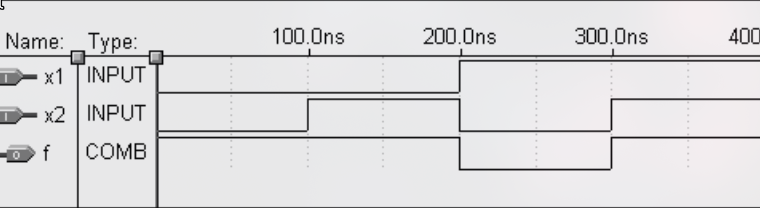
\includegraphics[scale=0.4]{figs/waveform.png}
            \label{stemplot}
          \end{figure}
          It is not suitable for larger circuits.
        \item \textbf{Schematic Capture}: Uses graphical symbols to represent logic gates and interconnections. Supports hierarchical design, where subcircuits are represented as symbols. One example of a circuit represented using Schematic Capture is,
          \begin{figure}[h!]
            \centering
            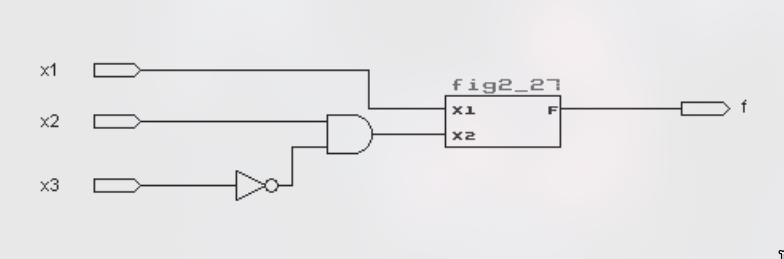
\includegraphics[scale=0.4]{figs/sc.png}
            \label{stemplot}
          \end{figure}
          It is a much better way of representing larger circuits, but its drawbacks are differences in UI, functionality of different software. This means repeated training when switching tools. Another drawback to note is that the GUI becomes awkward in case of larger circuits.
        \item \textbf{Hardware Description Languages (HDLs)}: They are similar to computer programming languages except, HDL's are used to describe hardware rather than software. Two HDL's are IEEE standard - \textbf{Verilog} and \textbf{VHDL}. In comparission to Schematic capture, a HDL such as verilog provies $portability$. This means that a circuit specified in Verilog can be implemented in different types of chips and with CAD tools provided by different companies, without having to change the Verilog specification. Both small and large logic circuit designs can be efficiently represented in Verilog code. Verilog has been used to define circuits such as microprocessors with millions of transistors. Verilog design entry can be combined with other methods. For example, a schematic-
          capture tool can be used in which a subcircuit in the schematic is described using Verilog.
      \end{enumerate}


      \subsubsection{Synthesis Process}
      Synthesis is the process of generating a logic circuit from a high-level description, such as a truth table, schematic, or Verilog code. CAD tools automate this process, which includes:
      \begin{itemize}
        \item Translating Verilog code or schematic diagrams into logic expressions.
        \item Generating logic equations from truth tables.
        \item Logic Optimization
      \end{itemize}

      \textbf{Logic Optimization}\newline
      The initial logic expressions provided by synthesis tools are often not optimal (reflecting on the designer's input). \textbf{Logic optimization} is a critical step where the synthesis tools manipulate these expressions to produce a more efficient circuit. Optimization goals depend on the design requirements and the target hardware technology. 

      \subsubsection{Functional Simulation}
      After completing design entry and synthesis, it is essential to verify that the designed circuit functions as expected. This is done using a \textbf{functional simulator}, which evaluates the circuit's behavior based on:
      \begin{itemize}
        \item Logic equations generated during synthesis (before optimization).
        \item Input valuations specified by the user.
      \end{itemize}
      The functional simulator:
      \begin{itemize}
        \item Applies input valuations to the logic equations.
        \item Computes the corresponding outputs.
        \item Presents the results as a truth table or timing diagram.
      \end{itemize}
      The user examines these results to ensure the circuit operates correctly.
      \textbf{Drawback: }The functional simulator assumes that the time needed for signals to propagate through the logic gates is negligible. In real logic gates this assumption is not realistic, regardless of the hardware technology chosen for implementation of the circuit.
      \subsubsection{Summary}
\begin{figure}[h!]
            \centering
            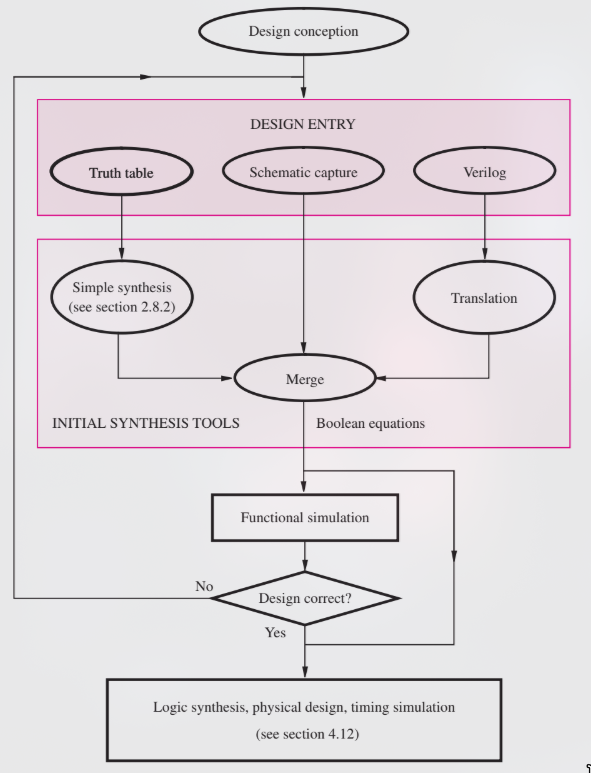
\includegraphics[scale=0.6]{figs/flowchart.png}
            \label{stemplot}
          \end{figure}  
          \end{document}
